\documentclass[letterpaper,twocolumn,10pt]{article}
\usepackage{usenix,epsfig,endnotes}
\usepackage{graphicx}
\usepackage{geometry}
\usepackage{lipsum}
\usepackage{fancyhdr}
\usepackage{hyperref}

\geometry{left=1in,right=1in,top=1in,bottom=1in}
\usepackage{titlesec}

\titleformat*{\section}{\Large\bfseries}
\titleformat*{\subsection}{\large\bfseries}
\renewcommand{\headrulewidth}{0pt}
\renewcommand{\footrulewidth}{1pt}  
\fancypagestyle{firststyle}
{
   \fancyhf{}
   \fancyfoot[L]{\footnotesize{FAWNLog code on github: \url{http://github.com/adegtiar/fawnlog}}}
}

\begin{document}
\date{}
\title{\LARGE \bf FAWNLog : A Low-Latency Shared Log on a Fast Array of Wimpy Nodes}

\author{
{\rm Alex Degtiar (adegtiar), Veronica Zheng (zhixingz), Junya Huang (junyah)}\\
Carnegie Mellon University}

\maketitle

% Use the following at camera-ready time to suppress page numbers.
% Comment it out when you first submit the paper for review.
\thispagestyle{firststyle}


\subsection*{Abstract}
FAWNLog is a system that organizes a cluster of wimpy flash nodes as a single low-latency shared log that can be accessed by multiple remote clients over the network. It is based on a system that supports such operations effectively with co-located clients, servers, and network-attached SSDs, but struggles in a wide area network context. FAWNLog introduces several techniques to reduce the latency in this context including: (1) avoiding message delays via parallel requests and flash unit prediction; (2) sequencer wait-and-timeout strategy to uniformly deal with prediction misses and enforce latency guarantees; and (3) flash unit support for improved hole detection and filling. Contributions 1 and 3 are made possible by the utilization of wimpy flash nodes, which enable support for multi-request joining, more sophisticated strategies for hole detection, and efficient management of hole metadata. Results show that FAWNLog can significantly reduce the latency  of requests in a WAN setting compared to its base system for a variety of workloads and without incurring significant overhead costs.

\section{Introduction}
A shared distributed log system built on top of a cluster of SSD nodes can be an important primitive for many distributed applications. CORFU is such system\cite{corfu}, and is shown to be an effective building block for applications such Tango\cite{tango}, an abstraction for shared data structures. These types of systems go a long way towards providing higher-level abstractions to build distributed system components such as consensus engines, databases, and transaction key-value stores.

However, CORFU was designed with the assumption that all components are co-located within a datacenter. While this captures a wide range of distributed applications, its high message delay overhead, a fundamental limitation of the client-centric design, means that clients cannot be separated from the rest of the system by a WAN without incurring large latency costs. This precludes the possibility of CORFU supporting possible applications such as automatic distributed stock purchasing, automatic saving of online game competition, and cross-region replicated database systems.

FAWNLog introduces a number of techniques to alleviate the high message delay overhead of CORFU. Latency reductions are accomplished by sending requests in parallel via flash unit prediction, having the sequencer buffer requests and create holes to ensure timely delivery, and by utilizing wimpy nodes as flash units, which allow for more sophisticated hole detection and request handling. In this paper, we describe CORFU and related system in greater detail, introduce the design and implementation of FAWNLog, and demonstrate the superior performance of the system against CORFU in WAN contexts.

\section{Background and related work}
\subsection{CORFU}
CORFU\cite{corfu} is a scalable distributed shared log system on a cluster of flash units. It ensures strong consistency among flash units of the shared log, which is essential for some distributed systems such as a consensus engine for consistent replication\cite{corfu} and an execution history for replica creation and geo-distribution\cite{seneca}. CORFU uses a sequencer for finding the tail of the shared log, and a replicated auxiliary for storing projections that maps addresses in the shared log to page numbers in a single flash unit. CORFU claims that the sequencer is not a single point of failure and the bottleneck for appending. Flash units in CORFU are only expected to have minimum functionality to satisfy system requirements. Thus, CORFU can be seen as a distributed SSD controller which provides an abstraction of a single huge SSD disk.

\subsection{FAWN}
FAWN\cite{fawn} is a cluster of local flash storage servers, with lower-power CPUs embedded. The architecture is aimed for parallel and data-intensive workloads, which often require fast random reads and sequential writes on the back-end storage system, but doesn't have complex logic involved and thus uses limited computation power. The poor performance of conventional HDD disks on large random reads workloads, along with high power energy cost of DRAM, make FAWN an attractive option for some of the current high-performance key-value storage system, such as Dynamo\cite{dynamo} in Amazon and memcached\cite{memcached} in Facebook. FAWN-KV\cite{fawn} is a specific key-value lookup system designed on FAWN to specifically support this kind of workloads.

\subsection{Tango}
Tango\cite{tango} provides an abstraction of replicated and in-memory data structures, and gets its atomicity, consistency, isolation and durability properties from the persistent distributed shared log, CORFU. Tango aims to efficiently design and manipulate metadata of distributed applications. Freedom on data structure design greatly expands the possible use scenarios of Tango, and provides a convenient tool for distributed applications. Tango also supports transactional access with high availability, which ensures its throughput to be competitive.

\section{Design and Implementation}
FAWNLog is an optimization based on CORFU\cite{corfu}. To compare our design with CORFU, we first implemented a subset of CORFU’s functionality. We needed a version that, while not optimized, fault-tolerant, or full-featured, could be a baseline to evaluate the relevant improvements of our techniques.

\subsection{Corfu}
There are three components in CORFU: client library, sequencer and flash units.

\subsubsection{Client library}
The client library provides append and read API. When append is called, the client interacts with the sequencer to get tokens and based on the projection to figure out which flash unit to communicate to. The client then make write requests to write to chosen flash unit on the offset indicated by the token. When read is called, the client figures out which flash unit to communicate to based on the projection mapping, and make read requests to chosen flash unit.

A projection is a mapping from the 64-bit virtual address in the shared log to a flash unit number and a page number pair. Thus, every token  corresponds to one page in the cluster. The translation works as follows: flash servers are divided into groups, then virtual addresses grow round-robin within each group and linearly between different groups. The number of flash units in a group could be configured to be different so that the effects of projection could be tested.

Holes can appear in the log when clients obtain tokens and then fail to use them immediately due to crashes or slowdowns. If a client encounters a hole when reading an unwritten position, it fills holes aggressively by sending a fill hole command to the flash unit. This kind of client read initiated hole filling reintroduces contention for log positions: if a client is merely late in using a reserved token and has not really crashed, it could end up competing with another client trying to fill the position.

\subsubsection{Sequencer}
To enforce global order of client write requests and eliminate client contention at the tail of the log, CORFU uses a dedicated sequencer which assigns clients “tokens” corresponding to tail log positions. The sequencer is implemented as a simple networked counter. To append data, the client first sends sequencer a get token request, the sequencer returns the current token value and increments the token. The client has now reserved a position in the log and can calculate the flash unit and offset it can write to based on the token. To support concurrent client requests, the sequencer uses a lock to protect the token.

\begin{center}
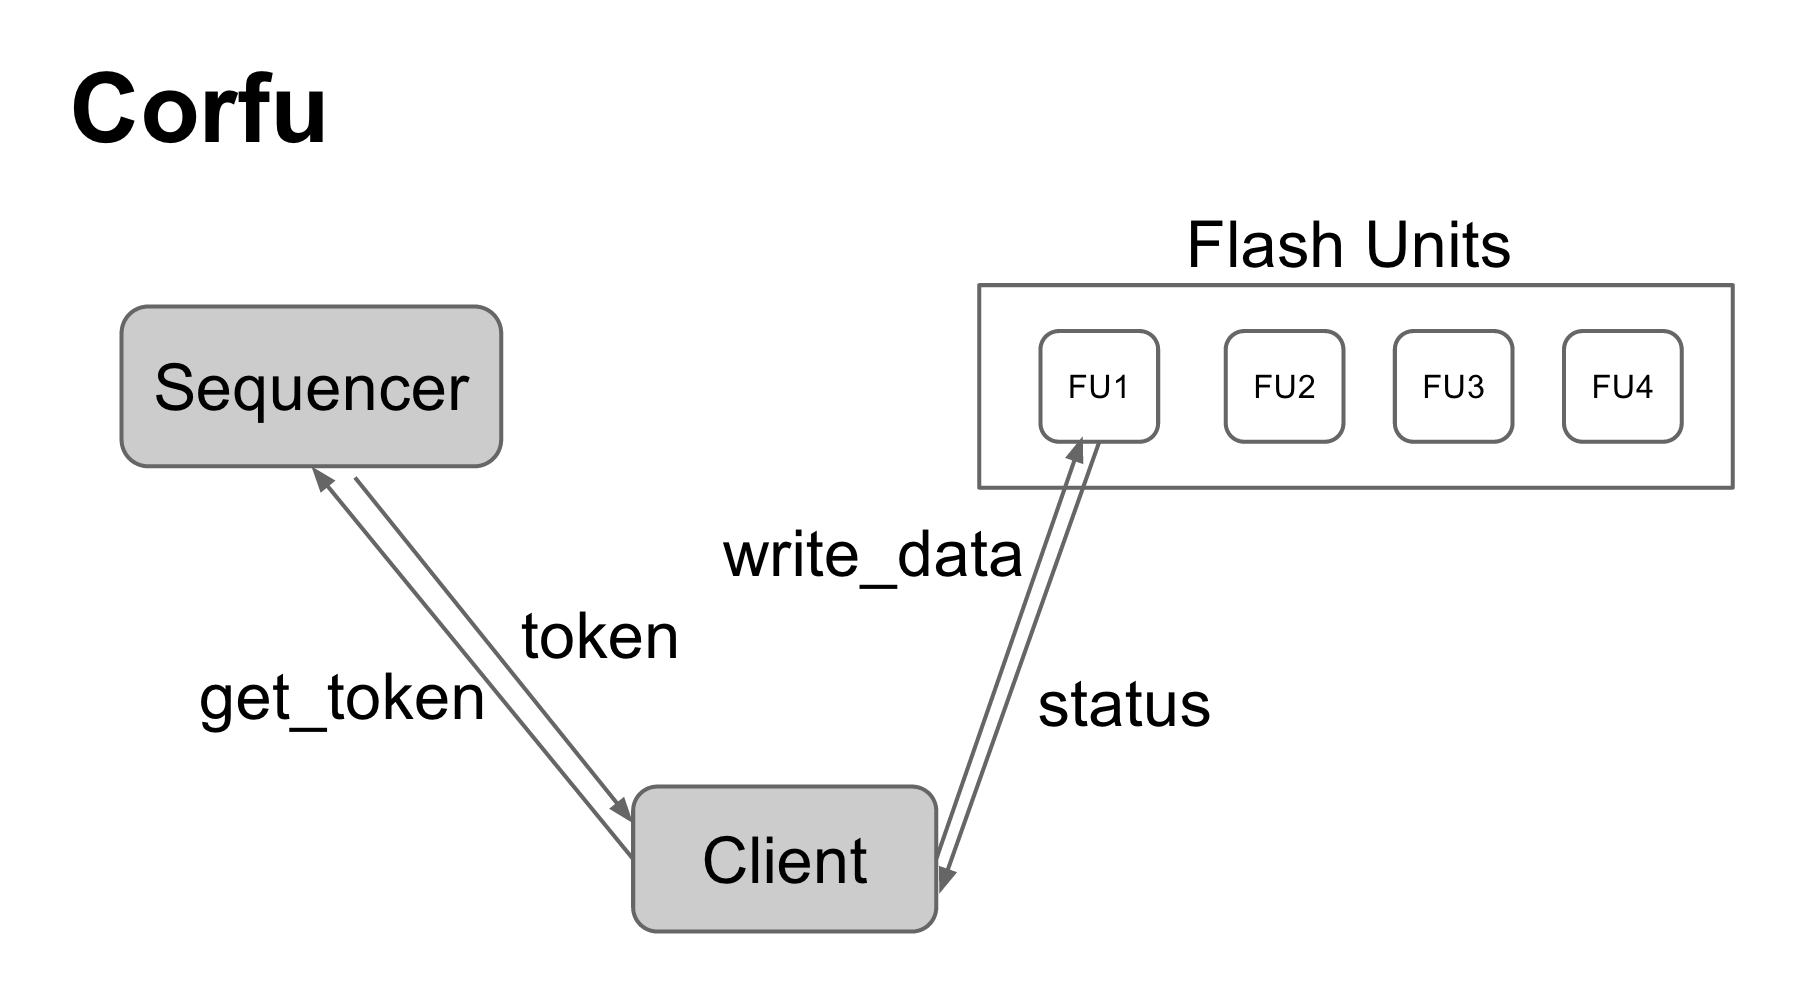
\includegraphics[width=.5\textwidth]{1.png}
\end{center}

\subsubsection{Flash unit}
The requirements for the flash unit are similar to those already supplied by a standard SSD, albeit with some minor discrepancies. The capacity of the flash is divided into fixed-size pages, each sequentially numbered within a logical address space. The flash pages should support write-once semantics over a read/write interface, where writing a page that’s already written or reading an unwritten page return errors. Other requirements besides these were out of the scope of this project and thus omitted. The implementation for this evaluation version of CORFU involved a file-backed interface to the SSD which maintained pages in sequential blocks of data + header, essentially interfaced with using appropriate pwrite/pread calls. Holes are stored via a simple header entry and filesystem sparse file support.

Protocol buffer based RPC are used for communications between client and sequencer, and between client and flash units.

\subsection{FAWNLog}
\subsubsection{Parallel requests}
CORFU needs two round trip time, one from client to sequencer and one from client to flash units to write data. Assuming sequencer and flash units are in the same data center or close to each other, the round trip time from client to sequencer and flash units are much larger than between sequencer and flash units. Rather than sending get token and receive token from sequencer, and then sending data to flash units, client can send get token request to sequencer and data to flash unit in parallel. And sequencer sends the offset for the data to the flash unit based on the token assigned to the request. When the client sends the request and data, it has to predict the current token in the sequencer and based on it to decide which flash unit to send the data to. If it sends to the wrong flash unit, it has to be cached in the flash unit to wait for its turn to write.

By making parallel requests, we reduce the delay from the two round trip time to the time the message travels from client to sequencer, the sequencer to flash unit, and the flash unit back to client. The token assigned by the sequencer corresponds to the offset in a particular flash unit. 

\begin{center}
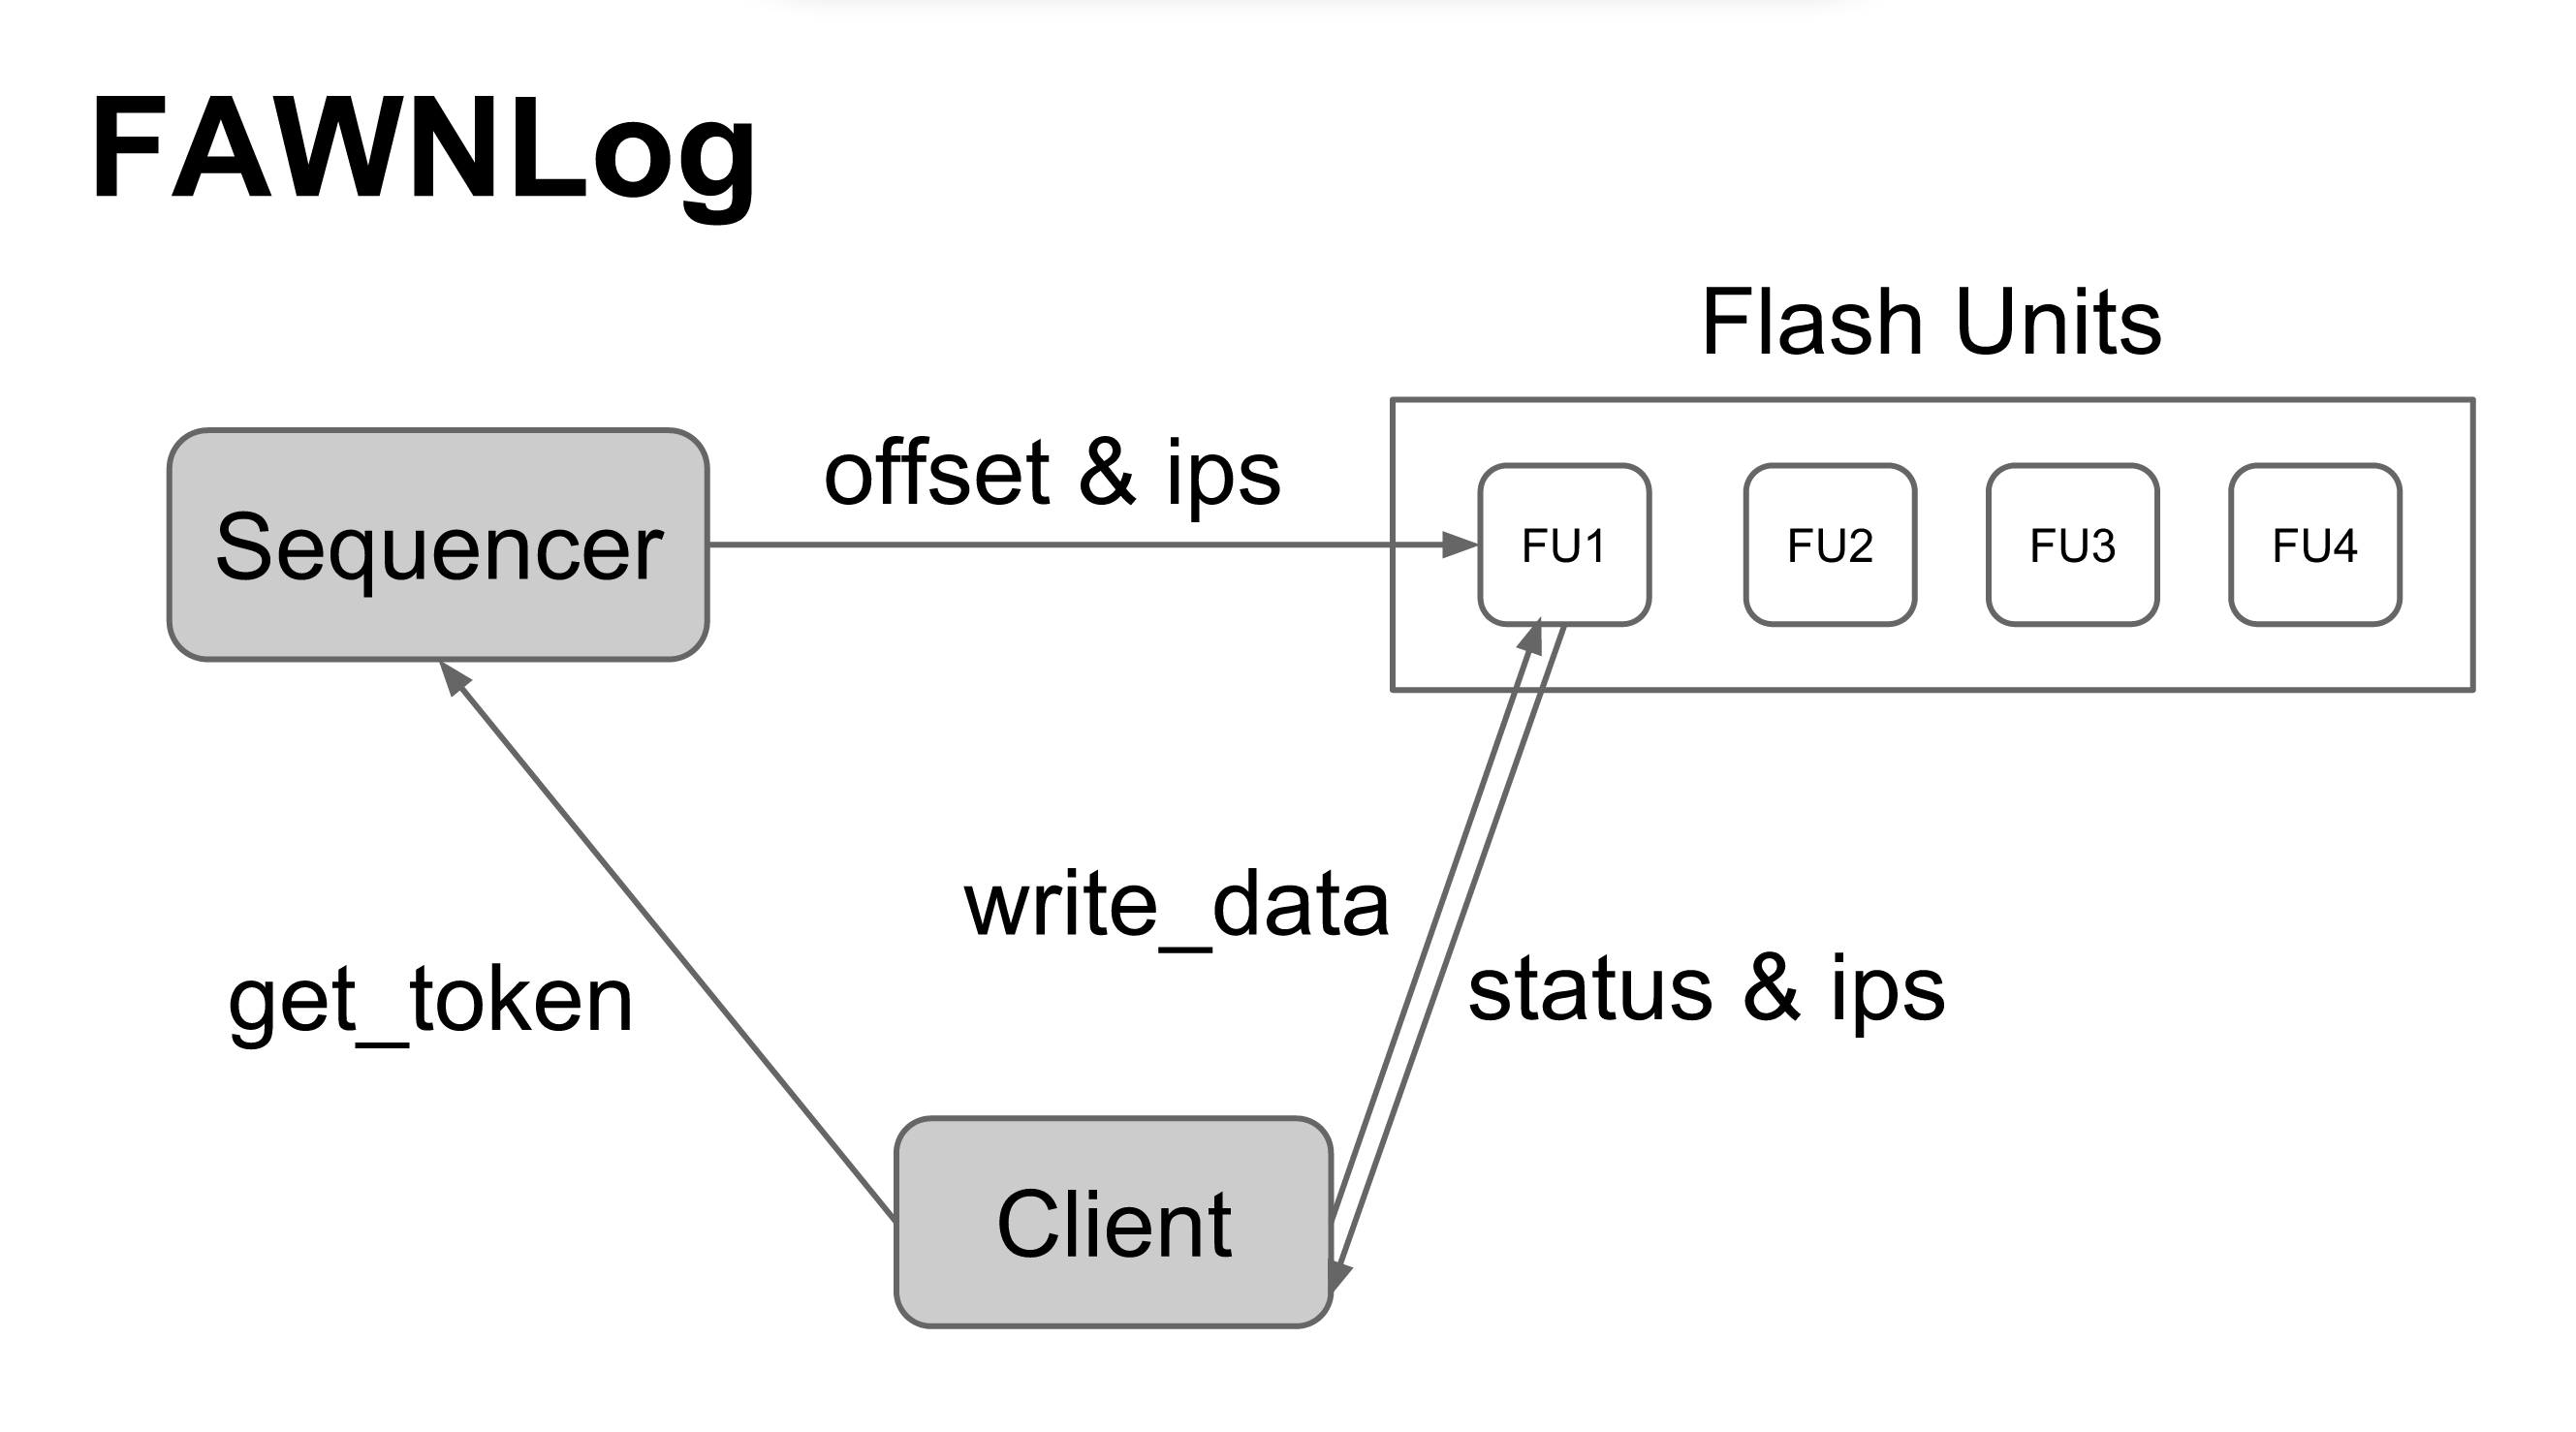
\includegraphics[width=.5\textwidth]{2.png}
\end{center}

\subsubsection{Sequencer wait and timeout strategy}
When a request arrives at the sequencer, the sequencer uses wait and timeout strategy to assign tokens. The sequencer then sends the offset which is calculated based on the token to the flash unit. Apart from the token, the sequencer maintains a table of queues for each flash unit and a cursor which points to the current flash unit the token corresponds to. Each time the sequencer increase the token, it also moves the cursor to point to the next flash unit. The request the client sends to the sequencer has data id which is a unique identifier identifies the data, and also a flash unit index which identifies the flash unit it sends data to. When sequencer gets the request, if the flash unit index in the request equals to the current cursor, it sends the request to the corresponding flash unit directly. Otherwise, it enqueues the request to the corresponding flash unit queue. The sequencer dequeues the request and sends it to the flash unit when the cursor moves to point to the corresponding flash unit. 

To bound how long the request is going to stay in the sequencer, the sequencer maintains a global request queue and a global request timer. When the sequencer enqueues a request to the flash unit queue, it also enqueues it to the global request queue. The sequencer sets the global request timer to timeout when the request at the head of the global request queue stays there for a certain time. When the global request timer fires, the sequencer removes the request at the head of the queue, and increments its token and cursor together so that the cursor will point to the flash unit in the request, and then sends the offset (token) to the flash unit. By doing this, the sequencer essentially created some holes in the token space which corresponds to holes in the address space in the flash units. The sequencer then sets the global request timer for the head of the current global request queue. The sequencer maintains a single global request timer for the head of the global request queue rather than a timer for each request is an optimization to reduce the sequencer overhead. 

\subsubsection{Flash unit prediction on the client}

Ideally, if the client knows the current value of the sequencer token and cursor, it can send the data to the corresponding flash unit. However, the client will not have this information and has to predict the current value of the sequencer token and sends the data to the corresponding flash unit based on the predication. If the prediction is incorrect, the request has to stay in the sequencer queues to wait for its turn. And if it stays for too long, it will trigger timeout and create holes. So the accuracy of the predication is important for reducing delay and holes created. 
\vspace{4cm}
\begin{center}
\begin{figure*}
  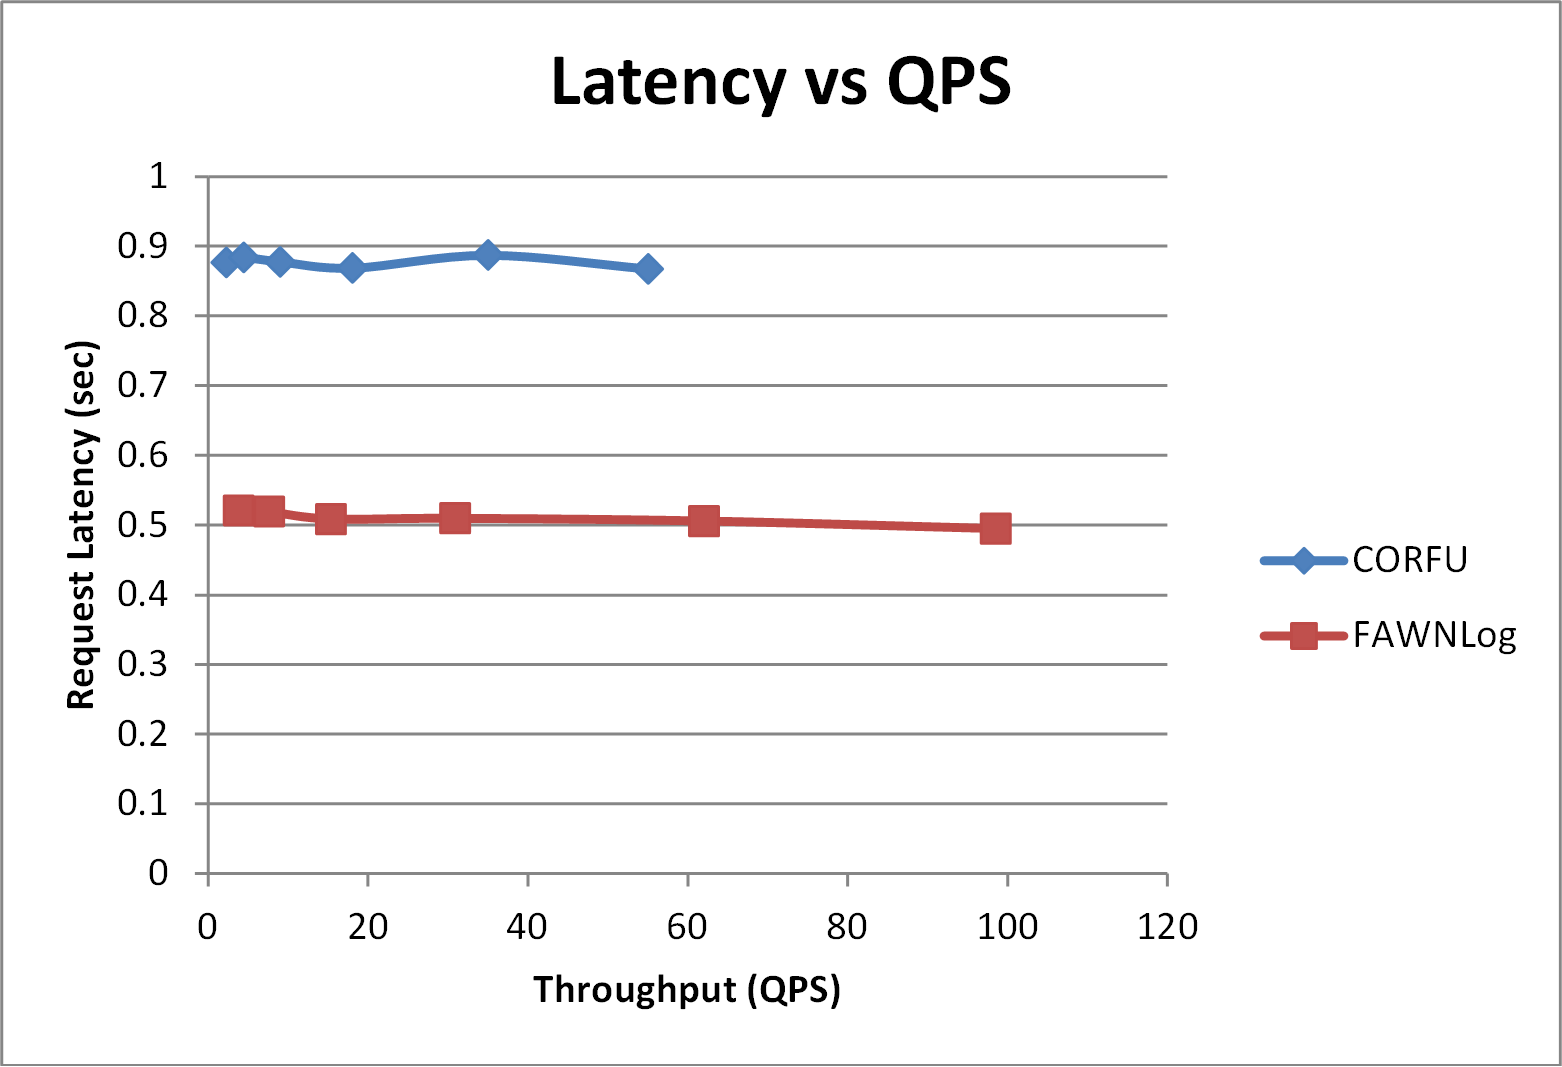
\includegraphics[width=\textwidth, height=10cm]{4.png}
  \caption{Test latency}
\end{figure*}
\end{center}

To help increasing client prediction accuracy, sequencer has a background thread calculating token increments per second (ips). When sequencer sends the data id and offset to the flash unit, it also attaches the ips information. And then the flash unit eventually forward this information to the client along with the result of the write. Client uses “last token + ips * (now - last token generated time)” to predicate the current token.

\begin{center}
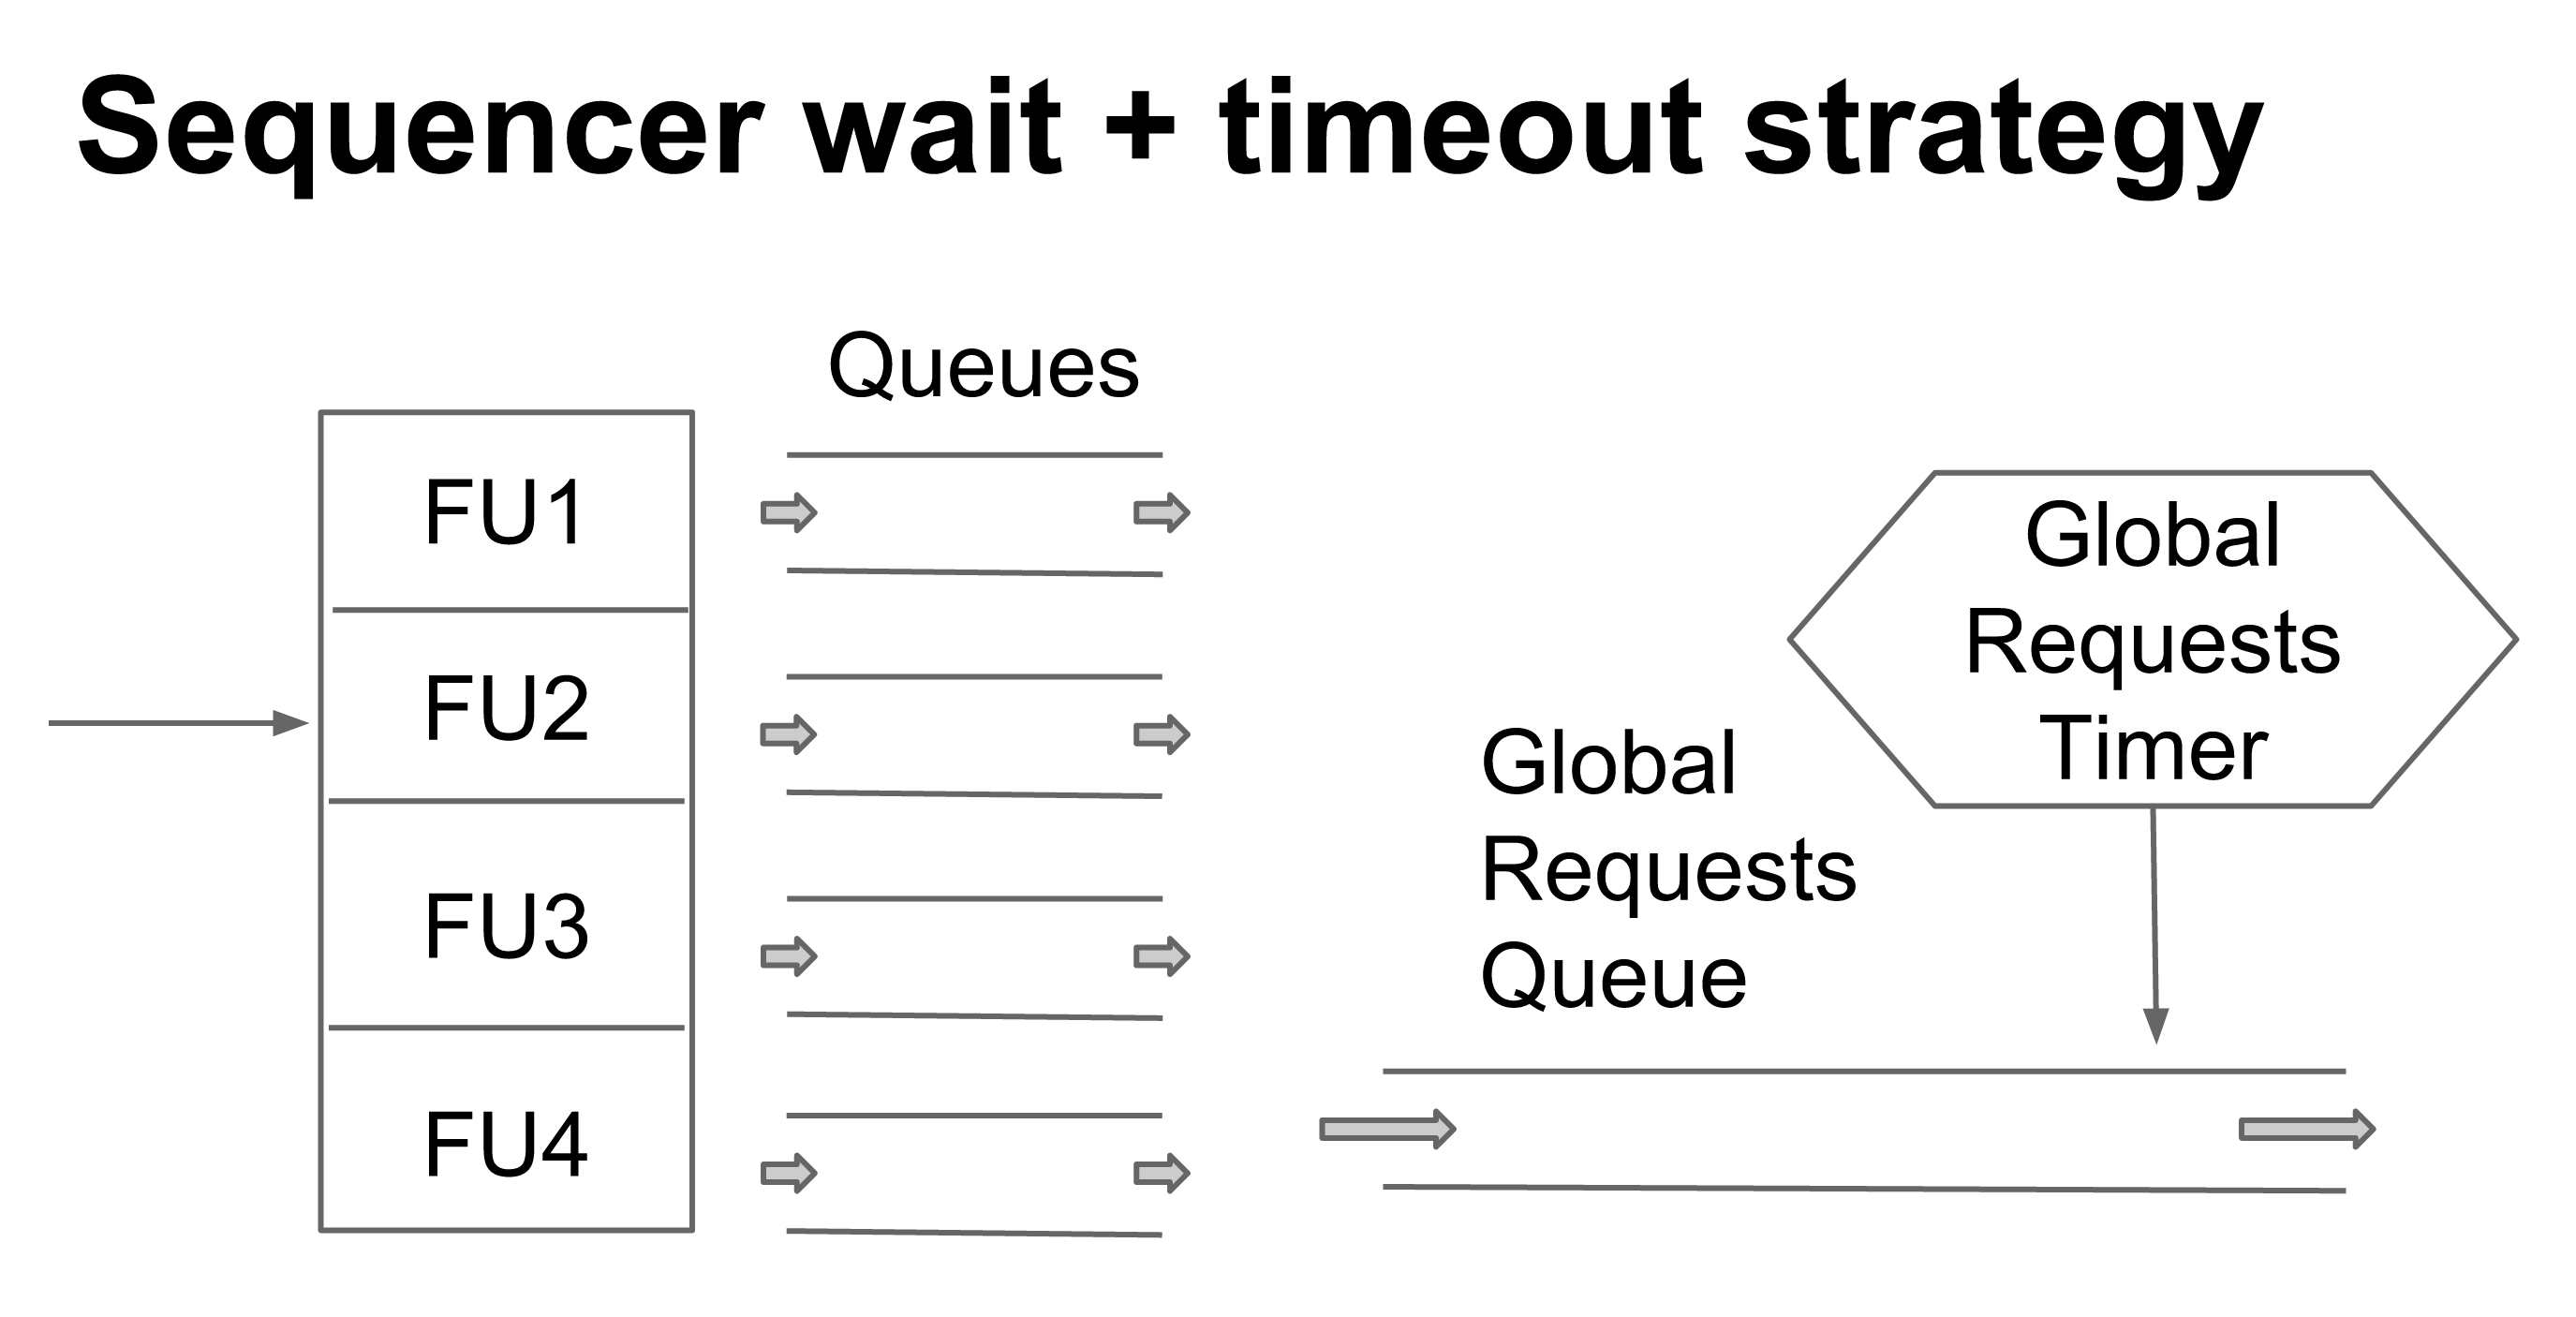
\includegraphics[width=.5\textwidth]{3.png}
\end{center}

In general, overpredict is better than underpredict. Because if the client overpredict the cursor by some number, it has to wait for the sequencer to increment the token by this number before the sequencer can fulfill its request. However, if the client underpredict the cursor by some number, it has to wait for the sequencer to increment the token by (total flash unit number - this number) before the sequencer can fulfill its request. Based on this observation, we conducted some experiments to record our prediction error distribution and fine tune the number we should overpredict.

\subsubsection{Hole detection/filling}
In CORFU, there is no ideal way to deal with client failures. If a client dies after requesting a token but before writing out a new page, a page is left allocated but not written. Having a value in a serialized log be undetermined can break sequential log semantics, so any indication of a potential hole is aggressively filled (either with junk or in flash unit metadata via special support) by any client which attempts to read this page. This can be a client latency/resource overhead to fill the hole, a contention overhead when client hole fills conflict with an in-progress append, and even further a waste if a client tries to fill a hole that simply hasn’t been written yet. These problems partly stem from a lack of knowledge and communication on the part of the CORFU clients.

In FAWNLog, a flash unit would likely have greater knowledge of (and greater locality to) the hole in question. If a client initializes a token sequencing but fails to write the page data to a flash unit, the flash unit would not only be aware of this information, but also of how long this hole has been left unwritten. As a result, a threshold can be configured to fill the hole and bound the contention between requests. Holes can be filled either immediately in reaction to client read requests, as a result of a background cleanup thread, or potentially via some other method.

\section{Evaluation and Results}

\subsection{Environment setup}
Since currently the FAWN cluster in lab is unaccessible, we choose Amazon Cloud Platform and the EC2 instances for experiments. The instance-type we are using is c3.xlarge, with two 40GB SSD and high network performance, for both sequencer and flash servers. Servers are set to the US West (Oregon) region, and the clients are set to the Asia Pacific (Sydney) region. We decide to separate them far in order to better explain and show our idea on latency comparison. We then setup every instance ready for experiments by using ssh and git.

\subsection{Test latency}
Since latency optimization is the most import improvement we make in FAWNLog, we test it under several different QPS (queries per second) values. The result (Figure 1) clearly shows that FAWNLog shortens nearly 50 percent of the original latency, which is one of the round trip time saved by making parallel requests. Due to some implementation details and time constraint, we are only able to test latency around a QPS of 60, but we think this is enough to show our ideas and thus decide to leave the time for other important tasks. 

\begin{center}
\begin{figure*}
  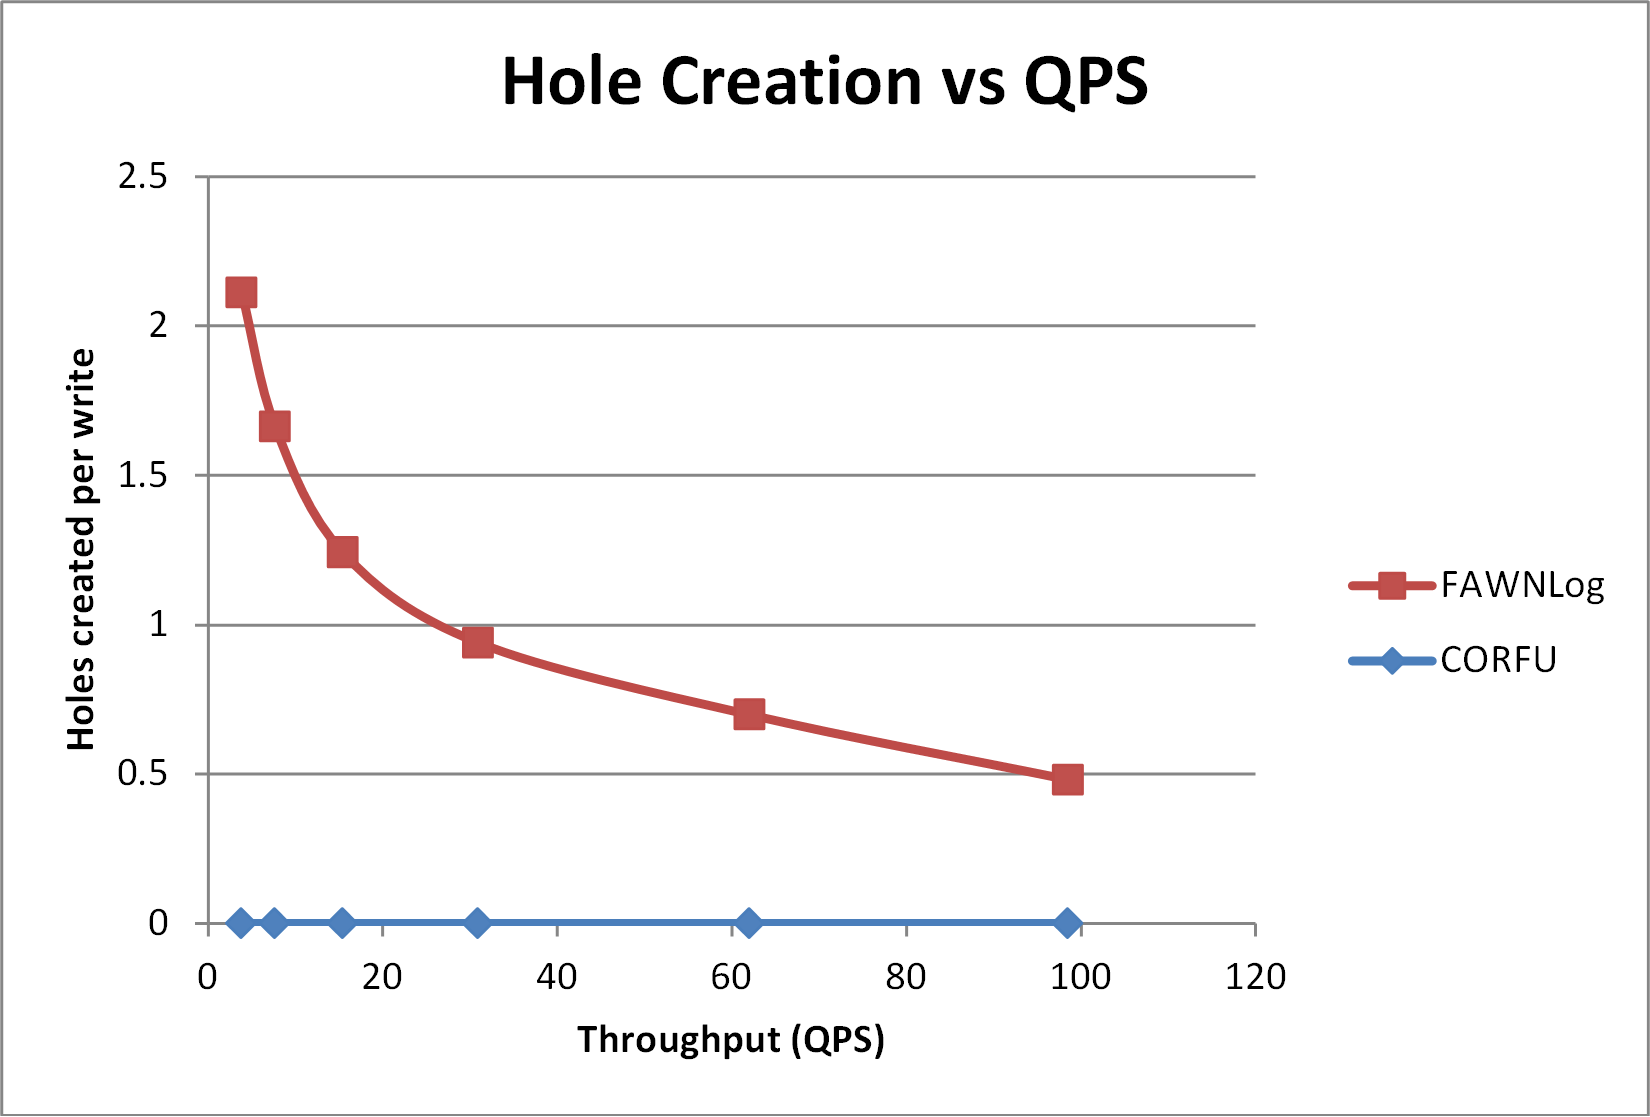
\includegraphics[width=\textwidth, height=10cm]{5.png}
  \caption{Test hole filling}
\end{figure*}
\end{center}

\subsection{Test hole filling}
The cost of our prediction is making holes in the shared log. Thus, measuring the speed of filling holes under different QPS is necessary to show that the additional capacity cost of our system is affordable. Figure 2 is the result of our experiments. It is important to note that holes made per write decreases obviously with the increase of QPS, which means that our system would incur very low capacity cost when used in real applications, where relatively high QPS is common. Even when QPS is low, the larger cost of making more holes won’t affect the whole performance of the application, because the number of queries is small and the capacity cost is in linear order of the number of queries.


\section{Conclusion}
FAWNLog provides an abstraction of a distributed shared log as CORFU\cite{corfu}, but has lower latency by making parallel requests and hole filling. It is more suitable for WAN setting.

FAWNLog reduces the latency of append from two round trip time (four one-way trip time) to three one-way trip time. It can significantly reduce the latency when client is far away from both sequencer and flash units, and the sequencer and flash units are close together. A possible setting will be the sequencer and flash units co-located in the same data center, while the clients are in other data centers far away. One alternative solution for such a setting is to deploy a proxy client co-located in the same data center with the sequencer and flash units. The proxy client can forward the client request to the sequencer, get the token back, send the data to flash units, and finally send the response back to the client. The proxy client acts exactly like the CORFU client. This solution can reduce the round trip time delay and very simple to deploy. However, FAWNLog has several advantages over this simple proxy client solution. First, the sequencer and flash units can be distributed in different places. For example, we can have multiple flash clusters for multiple databases replicated in different regions. The sequencer cannot be co-located with all flash units. Using a proxy client won’t be possible in this scenario. We can still reduce the latency by using FAWNLog’s parallel requests sending strategy. In addition, the techniques introduced in FAWNLog preclude the need for a potentially expensive cluster of proxy clients, which may not always be worth the cost of provisioning and running additional machines. Especially considering the goal to use wimpy clusters is to reduce cost and save energy.

In CORFU and FAWNLog design, the sequencer is eventually going to be a bottleneck when scaling the system. In CORFU, the sequencer logic is extremely simple. It only returns its current token value when receiving get token request and increments its token. In FAWNLog, to reduce latency, we implemented parallel requests and sequencer wait-and-timeout strategy. We argue that the overhead FAWNLog added to the sequencer is so small that it will not restrict the sequencer bottleneck too much when scaling the system. When sequencer becomes a bottleneck, the system is under high query per second (QPS). Under high QPS, the FAWNLog global request timer will never be triggered, the only overhead FAWNLog added to the sequencer is enqueuing the request and dequeuing the request before and after incrementing the token. 

{\footnotesize \bibliographystyle{abbrv}
\bibliography{sample}}

\end{document}







